\documentclass[a4paper,12pt,russian]{article} %размер листа и размер шрифта
\usepackage[left=3cm,right=3cm, top=3cm, bottom=3cm, bindingoffset=0cm]{geometry}
%\usepackage[margin=1.25in]{geometry}
\pagestyle{plain} %включаем нюмерацию страниц
\usepackage{amsmath,amssymb,amsthm,enumitem,amsfonts, amscd, array,graphicx,wrapfig}
\usepackage[T2A]{fontenc}
\usepackage[utf8]{inputenc}
\usepackage[russian]{babel} %переносы слов
%\usepackage[sort]{natbib}
%\usepackage[colorlinks,allcolors=blue]{hyperref}
%\usepackage[small,bf]{titlesec}
%\titlelabel{\thetitle.\hspace{0.5em}}
%\PassOptionsToPackage{usenames,dvipsnames}{xcolor}
%\usepackage{tikz}
\usepackage{mathtools}
\usepackage{cmap}
\usepackage{hyperref}
\usepackage{xcolor}
\hypersetup{
  unicode=true, % закладки для текстов в юникоде
  colorlinks=true, % цветные ссылки
  linkcolor=blue, % цвет гиперссылок внутри документа
  citecolor=teal, % цвет библиографических ссылок
  urlcolor=red % цвет ссылок на ресурсы в сети
}
 
%\usepackage[usenames]{color}
\usepackage{colortbl}
\usepackage[nottoc,numbib]{tocbibind}
\usepackage{indentfirst} %отступ в первом абзаце

%\DeclareMathOperator*{\argmax}{argmax}

\theoremstyle{definition}
\newtheorem{exercise}{Задача}
\newtheorem{definition}{Определение}

%\theoremstyle{theorem}
\newtheorem{theorem}{Теорема}
\newtheorem{lemma}{Лемма}
\newtheorem{proposition}{Утверждение}
\newtheorem{cor}{Следствие}
\newtheorem{remark}{Замечание}
\newtheorem{quest}{Вопрос}

\newenvironment{thproof}[1][\proofname]{%
  \proof[\rmfamily \upshape \bfseries #1]%
}{\endproof}






\newcommand{\floor}[1]{\lfloor{#1}\rfloor}
\newcommand{\ceil}[1]{\lceil{#1}\rceil}
\DeclareMathOperator{\E}{E}
\DeclareMathOperator{\Var}{Var}
\DeclareMathOperator{\I}{I}
\DeclareMathOperator{\sgn}{sgn}
\DeclareMathOperator{\Law}{Law}
\DeclareMathOperator{\argmax}{arg\,max}
\renewcommand{\hat}{\widehat}
\renewcommand{\tilde}{\widetilde}
\renewcommand{\epsilon}{\varepsilon}
\renewcommand{\P}{\mathrm{P}}
\newcommand{\F}{\mathcal{F}}
\newcommand{\R}{\mathbb{R}}
\newcommand{\bt}{\tilde{b}}
\renewcommand{\b}{\bar b}
\newcommand{\M}{\mathcal{M}}
\let\Ss\S
\renewcommand{\S}{\mathcal{S}}
\newcommand{\cadlag}{c\`adl\`ag}




\title{Стратегия оптимального роста в многоагентной модели рынка с афинными выплатами}
\author{}
\date{}

\begin{document}

\begin{center}
    \footnotesize{ФЕДЕРАЛЬНОЕ ГОСУДАРСТВЕННОЕ БЮДЖЕТНОЕ ОБРАЗОВАТЕЛЬНОЕ}\\ 
    \footnotesize{УЧРЕЖДЕНИЕ ВЫСШЕГО ОБРАЗОВАНИЯ}\\
    \small{\textbf{«МОСКОВСКИЙ ГОСУДАРСТВЕННЫЙ УНИВЕРСИТЕТ}}\\
    \small{\textbf{имени М.В.ЛОМОНОСОВА»}}\\
    \hfill \break
    \normalsize{МЕХАНИКО-МАТЕМАТИЧЕСКИЙ ФАКУЛЬТЕТ}\\
     \hfill \break
    \normalsize{КАФЕДРА ТЕОРИИ ВЕРОЯТНОСТЕЙ}\\
    \hfill\break
    \hfill \break
    \hfill \break
    \large{ВЫПУСКНАЯ КВАЛИФИКАЦИОННАЯ РАБОТА}\\
    \large{(ДИПЛОМНАЯ РАБОТА)}\\
    \large{специалиста}\\
    \hfill \break
    \hfill \break
    \textbf{Стратегия оптимального роста в многоагентной модели рынка с афинными выплатами}\\
\end{center}
    \hfill \break
    \hfill \break
    
    \hfill
\begin{tabular}{@{}l@{}}
    Выполнила студентка\\
    609 группы \\
    \textbf{Токаева Александра Александровна} \\
    \hfill \\
    \hfill \\
    \underline{\hspace{3cm}} \\
    подпись студента \\
    
    \hfill \\
    \hfill \\
    
    Научный руководитель: \\
    к.ф.-м.н. \textbf{Житлухин Михаил Валентинович} \\
    \hfill \\
    \hfill \\
    \underline{\hspace{3cm}} \\
    подпись научного руководителя \\
\end{tabular}
    
    \hfill \break \\
    \hfill \\
    \hfill
    
\begin{center}
    Москва\\
    2023
\end{center}
    \thispagestyle{empty} % выключение отображение номера для этой страницы
    
    %Содержание
    \tableofcontents
    
    \newpage
    
\section{Введение}
Основным предметом исследования в данной работе является стохастическая модель финансового рынка с дискретным временем, описывающая конкуренцию агентов (инвесторов) за несколько активов на бесконечном горизонте времени. Выплаты активов делятся между инвесторами пропорционально доле капитала, вложенного инвестором в этот актив. Цены на рынке задаются эндогенно из условия краткосрочного равенства спроса и предложения для каждого из активов. Как следствие, прибыль или убыток инвестора зависит не только от реализовавшихся выплат активов, но и от действий остальных инвесторов.

Основная цель работы — нахождение стратегии, называемой стратегией оптимального относительного роста (или лог-оптимальной). Суть этой стратегии заключается в том, что логарифм относительного капитала использующего эту стратегию инвестора является субмартингалом вне зависимости от того, какие стратегии используют остальные инвесторы. Под относительным капиталом мы понимаем долю капитала инвестора от общего капитала на рынке.

Хорошо известно, что в стандартных моделях рынка  субмартингальное свойство стратегии влечет за собой ряд оптимальных свойств (см.\cite{AlgoetCover1988}, \cite{KaratzasKardaras2007}). В нашей модели найденная стратегия также окажется оптимальной в следующем смысле: относительный капитал использующего эту стратегию инвестора остается отделенным от нуля с вероятностью один. Кроме того, мы покажем, что если репрезентативная стратегия остальных инвесторов асимптотически отличается от оптимальной стратегии, то доля капитала инвестора с оптимальной стратегией стремится к единице.

Модель, изучаемую в работе, в общих словах можно описать следующим образом. На рынке присутствуют $K$ активов, выплачивающих дивиденды в дискретные моменты времени, а также $N$ агентов, которые могут покупать и продавать активы и получать выплачиваемые дивиденды (но короткие продажи запрещены). С течением времени капитал инвесторов изменяется за счет получения дивидендов (подчеркнем, что активы короткоживущие, поэтому агент не получает прибыль от изменения цены актива на длинном горизонте - потому что актив живет только на протяжении одного временного промежутка). В целом, такая модель во многом схожа со стандартными моделями финансовой математики, с той лишь разницей, что в нашей модели цены активов определяются не экзогенно, а эндогенно, а именно, стратегиями инвесторов. Другими словами, в нашей модели мы считаем, что предложение каждой акции фиксировано (и, без ограничения общности, равно единице), а цена акции должна быть такой, чтобы спрос инвесторов оказался равен предложению.

Эта задача является продолжением исследований в области теории оптимального роста. Первыми работами в этом направлении были \cite{Kelly1956}, \cite{Breiman1961}, где были найдены асимптотически оптимальные стратегии для моделей с дискретным временем. Далее эти результаты были значительно улучшены. Среди множества работ можно выделить \cite{AlgoetCover1988}, где была рассмотрена общая модель с дискретным временем. Однако в этой работе дивиденды задавались экзогенно и, кроме того, рассматривалась задача одного инвестора, а не задача конкуренции инвесторов.

Наша модель обобщает модель \cite{Amir2013}, где исследовались оптимальные стратегии в модели рынка с короткоживущими активами в дискретном времени. В нашей модели предполагается аффинная структура выплат активов, что существенно осложняет нахождение оптимальной стратегии. Также стоит отметить статью \cite{Drokin-Zhitlukhin2020}, в которой тоже обобщается модель из \cite{Amir2013}, но другим способом: добавлением к короткоживущим активам безрискового актива (банковского счета). Последние достижения в области Эволюцинных финансов представлены в \cite{EvstigneevEvolFinance2016}, \cite{Holfort2019}.

Таким образом, наша модель в дискретном времени обладает следующими особенностями: 

1) мы расссматриваем не  действия одного (не влияющего на цены) инвестора против всего остального рынка, а игру нескольких агентов, в которой каждый агент имеет свою стратегию, каждая из которых оказывают влияние на цены активов, что существенно усложняет 
поиск оптимальной стратегии.

2) Активы в нашей модели короткоживущие в том смысле, что они 
выпускаются в момент $t$, в момент $t+1$ выплачивают дивиденды в соответствии с формулой, которая будет дана ниже, и исчезают. Другими словами, короткоживущие активы нельзя продать 
в момент $t+1$, от них можно только получить дивиденды.

3) Дивиденды задаются экзогенно, а цены активов определяются эндогенно из условия равенства спроса и предложения. Отметим, что в нашей модели действия инвесторов предшествуют установлению цен, то есть сначала инвесторы объявляют, какую долю своего капитала они хотят вложить в каждый из активов, а после этого цены устанавливаются из условия равенства спроса и предложения. Несмотря на то, что он является упрощением реально наблюдаемой на рынке ситуации, этот подход экономически обоснован (см.\cite{Shapley-Shubik1977}).

4) Размер дивидендов, выплачиваемых активом, зависит от объема капитала, который в него суммарно вложили все инвесторы на предыдущем шаге. Это экономически обоснованно, поскольку чем больше в компанию вложили, тем больше у нее возможностей для развития и, соответственно, для выплаты больших дивидендов. Отметим, что именно эта зависимость от объема вложенного капитала (который, в свою очередь, зависит от стратегий агаентов) отличает нашу модель от других и делает нашу задачу сложной.

5) Наша модель развивает подход, предложенный в \cite{Amir2013}, где также рассматривались оптимальные стратегии в модели с несколькими активами и эндогенными ценами в дискретном времени, но величина дивидедов актива не зависела от объема вложенного в актив капитала.
Именно поэтому в модели \cite{Amir2013} удалось найти оптимальную стратегию в явном виде.
В нашем же случае мы не найдем явный вид оптимальной стратегии, но докажем ее существование и асимптотическую оптимальность. Найденная нами стратегия 
будет зависеть от текущих капиталов инвесторов, которые в свою очередь зависят от их прошлых действий, в то время как в \cite{Amir2013} оптимальная стратегия не зависела
от прошлых действий инвесторов. При этом в частном случае нашей модели, соотвествующем модели \cite{Amir2013}, найденная нами стратегия окажется в точности стратегией из \cite{Amir2013}.

Основной результат работы состоит в доказательстве существования 
стратегии оптимального относительного роста (или лог-оптимальной стратегии). 
Будет показано, что пропорция капитала, которую эта стратегия вкладывает 
в актив $k=1,2$, задается неявно как неподвижная точка отображения

\begin{equation*}
    L_{t}^k(\lambda^*, \bar s_t,\bar\chi_t) 
= \E_t\left(
  \frac{g_{t+1}^k(\lambda^*,\bar s_{t+1},\bar\chi_t)}
       {\sum_{k=1}^K g_{t+1}^k(\lambda^*,\bar s_{t+1},\bar\chi_t)} 
  \right).
\end{equation*}



Дипломная работа организована следующим образом. В разделе~\ref{section2-model} описывается
общая модель рынка с эндогенными ценами. В разделе~\ref{section3-main-results} даются определения выживающей и лог-оптимальной стратегии, а также формулируются основные результаты об ее сущестововании и асимптотическом поведении. В разделе~\ref{section4-example} приводится численный пример, демонстрирующий поведение выживающей стратегии на рынке. В разделе~\ref{section5-relation-to-other-models} показывается связь результатов в нашей модели с результатами в других известных моделях. Раздел~\ref{section6-proofs} содержит доказательства основных результатов. Раздел~\ref{section7-conclusion} подводит итог работы.

\section{Модель рынка}\
\label{section2-model}
В данном разделе будет предложена общая модель рынка с 
произвольным числом агентов и активов. В дальнейшем, однако, будет рассматриваться только частный случай двух агентов и двух активов.

Пусть $(\Omega,\F,\P)$ — вероятностное пространство с полной дискретной фильтрацией $\mathbb{F} = (\F_t)_{t\ge 0}$.

Рынок в модели состоит из $N\ge 2$ агентов и $K\ge 2$ короткоживущих активов. В каждый из моментов времени $t=0,1,\dots$ на рынке "рождается" одна единица каждого из $K$ активов, а инвесторы одновременно и независимо принимают решение о том, в каких долях они инвестируют свой капитал в каждый из $K$ активов на промежутке от $t$ до $t+1$. Цена на каждый из активов в момент $t$ устанавливаяется эндогенно из условия равенства спроса и предложения в момент $t$. После этого в момент $t+1$ каждый из активов выплачивает дивиденды в соответствии с формулой, которая будет дана ниже. Эти дивиденды распределяются между инвесторами пропорционально капиталу, который они инвестировали в данный актив. После выплаты дивидендов все активы умирают и рождаются заново, и процедура определения цены происходит опять. 

Рынок эволюционирует под влиянием случайного фактора (возможно, многомерного), который моделируются посредством случайных величин $s_1, s_2, \dots$ из измеримого множества $\Omega$. Случайная величина $s_t$ интерпретируется как состояние рынка в момент времени $t$.

Агент $n$, где $n=1,\ldots,N$, характеризуется своим неслучаным начальным капиталом $W^n_0 >0$ и стратегией $\Lambda^n$. Капитал $W_t^n$ $n$-го агента в произвольный неначальный момент $t$ определяется из динамики, которая будет приведена ниже, и образует $\mathbb{F}$-измеримую случайную последовательность капиталов $W^n = (W_t^n)_{t=0}^\infty$.

В каждый момент времени $t$ каждый агент $n$ выбирает вектор долей $\lambda_t^n = (\lambda_{t}^{n,1},\ldots,\lambda_{t}^{n,K})$, в которых он вкладывает свой капитал $W_t^n$ в каждый из $K$ активов в момент времени $t$ (в нашей модели агент обязан вложить весь свой капитал в активы, банковского счета нет). Например, сумма $\lambda_{t}^{n,k} W_t^n$ тратится агентом $n$ на покупку актива $k$ (а сколько именно единиц актива $k$ этот агент купил — будет определено, когда все агенты объявят, сколько денег они выделили на покупку актива $k$, и из краткосрочного равенства спроса и предложения определится цена данного актива).

Доли $\lambda_t^n$ для разделения капитала могут зависеть от истории состояний случайного фактора $\bar s_{t-1} := (s_1,...,s_{t-1})$,  вектора начальных капиталов $ \bar W_0 := (W_0^1,...,W_0^N)$ и истории стратегий всех агентов 
$\bar \lambda_{t-1} := ( \lambda_0,..., \lambda_{t-1})$, где $ \lambda_s = (\lambda^1_s, \dots, \lambda^N_s )$.

Стратегия $n$-го агента — это последовательность $\Lambda^n =
(\Lambda_t^n)_{t=0}^\infty$ векторнозначных функций 
\[
\Lambda_t^n =\Lambda_t^n(\bar s_{t},\bar W_0 , \bar \lambda_{t-1})
\]
со значениями в стандартном $K$-симплексе 
\[
\Delta_K
=\{ (a^1, \dots, a^K) \in \R^K_+ : a^1+\ldots+a^K = 1\}
\]
и измеримых относительно \textcolor{red} { {$\F_t\otimes \mathcal{B}(\R_+)$}.  - что тут надо поставить? Тут же не от одного омега теперь завивимость, а от последовательности, и еще от последовательности лямбд?} 

Для $k=1,\ldots,K$, $k$-я координата $\Lambda_t^{n,k}$ соответствует доле капитала, которую 
$n$-й агент вложил в покупку $k$-го актива в момент времени $t$. Короткие продажи запрещены.
Для $t=0$, функция $\Lambda_0^n = \Lambda_0^n(\bar W_0)$ не зависит от истории состояний случайного фактора и истории стратегий агентов.

Зависимость $\Lambda_t^n$ от  $\bar \lambda_{t-1}$ нельзя опустить, потому что построенная нами оптимальная стратегия будет зависеть от полного капитала рынка, который, в свою очередь, зависит от $\bar \lambda_{t}$. \textcolor{red} {Это правильная фраза? Или почему нельзя опустить? И тут $\lambda_{t-1}$ или $\lambda_t$ должно быть?}

Если заданы вектор начальных капиталов $\bar W_0=(\bar W_0^1,\ldots, \bar W_0^N)$ и профиль стратегей $\Lambda=(\Lambda^1,\dots,\Lambda^N)$, то инвестиционные стратегии каждого агента на этом рынке определяются следующим рекурсивным соотношением: 
\begin{equation}
\label{1-realization-of-strategy}
\lambda_0^n = \Lambda_0^n(\bar W_0), \qquad
\lambda_t^n(\bar s_{t}) = \Lambda_t^n( \bar s_{t}, \bar W_0, \bar \lambda_{t-1}( \bar s_{t-1})),\ t\ge 1,
\end{equation}
где  $ \bar \lambda_{t}( \bar s_{t})) = ( \lambda_0, \lambda_{1}(\bar s_{1})),\dots, \lambda_{t}(  \bar s_{t}) ))$.
Далее мы будем опускать зависимость от  $\bar s_{t}$, где это не будет приводить к неоднозначности.  


Обозначим за $\bar P_t = (P_{t}^1,\ldots,P_{t}^K)$ вектор цен активов в момент времени $t$.
Коррдината $P_{t}^k$  соответствует цене одной единицы актива $k$ в момент $t$.
Зададим динамику капитала $W_t^n = W_t^n(  \bar s_{t} )$ $n$-го агента и вектора цен $\bar P_t= \bar P_t( \bar s_{t} )$ для заданного профиля стратегий $\Lambda=(\Lambda^1,\dots,\Lambda^N)$ и вектора начальных капиталов $\bar W_0$.

Цены формируются из условия равенства спроса и предложения в каждый момент времени. 
Состав портфеля агента $n$ в момент времени $t\ge0$ характеризуется вектором $ \bar X_t^n=(X_{t}^{n,1},\dots,X_{t}^{n,K})$, где $X_{t}^{n,k}$ есть количество единиц актива $k$ в портфеле.
Скалярное произведение $\langle \bar P_{t}, \bar X_{t}^{n}\rangle=\sum_{k=1}^{K}P_{t}^k X_{t}^{n,k}$ показывает цену всего портфеля агента $n$ в момент времени $t$.

В момент времени $t=0$ капитал $n$-го агента равен его неслучайному начальному капиталу $W_{0}^{n}$.
За $A_{t}^k = A_{t}^k(  \bar s_{t} )$, $k=1,\dots,K$,  обозначим величину дивидендов, которые единица актива $k$ выплачивает в момент времени $t\ge 1$. Поскольку мы предполагаем, что на рынке количество каждого актива равно единице, то величина $A_{t}^k$ характеризует полную выплату дивидендов от актива $k$. Тогда величина капитала $n$-го агента 
в момент времени $t\ge1$ равна
\begin{equation}
W_{t}^{n}=\langle \bar A_{t}, \bar X_{t-1}^{n}\rangle=\sum_{k=1}^{K}A_{t}^k X_{t-1}^{n,k},
\label{2-W-t-n}%
\end{equation}
То есть величина капитала в момент времени $t$ формируется из выплат акций, купленных в мемент времени $t-1$.

Если агент $n$ вложил долю $\lambda_{t,k}^n$ своего капитала в покупку актива $k$ в момент $t$, тогда число единиц актива, который он купил, равно
\begin{equation}
X_{t}^{n,k} = \frac{\lambda_{t}^{n,k} W_t^n}{P_{t}^k}. \label{3-X-t-n-k}
\end{equation}
Напомним, что каждого актива на рынке ровно 1 единица, и при этом цены устанавливаются такие, чтобы спрос был равен предложению, тогда для всех $t\ge0$ и $k=1,\dots,K$ выполнено:
\[
1 = \sum_{n=1}^{N}X_{t}^{n,k} 
= \sum_{n=1}^{N}\frac{\lambda_{t}^{n,k}W_{t}^{n}}{P_{t}^k}= \frac{1}{P_{t}^k} \sum_{n=1}^{N}\lambda_{t}^{n,k}W_{t}^{n}, 
\]
Отсюда находим, что установившиеся равновесные цены имеют вид
\begin{equation}
P_{t}^k = \sum_{n=1}^{N}\lambda_{t}^{n,k}W_{t}^{n}. \label{4-P-t-k}
\end{equation}
Если правая часть этого выражения равна нулю на множестве  $\bar s_{t} $, то в формуле \eqref{3-X-t-n-k} полагаем $X_{t}^{n,k}=0$ на этом множестве. \textcolor{red} { а что, там разве и так ноль не будет, если справа ноль?} 

Таким образом, имея профиль стратегий $\Lambda=(\Lambda^1,\dots,\Lambda^N)$ и вектор начальных капиталов, мы можем рекурсивно с помощью выражений \eqref{2-W-t-n}--\eqref{4-P-t-k} восстановить случайную траекторию системы, задаваемой последовательностями капиталов агентов $W_t^n$ , равновесных цен $ \bar P_t=(P_{t}^1,\dots,P_{t}^K)$ и составов портфелей $X_t^n=(X_{t}^{n,1},\dots,X_{t}^{n,K})$.

В частности, используя \eqref{2-W-t-n}--\eqref{4-P-t-k}, получаем, что последовательность капиталов $W_t^n$ удовлетворяет соотношению
\begin{equation}
\label{5-dynamics-of-W}
W_{t+1}^n = \sum_{k=1}^K 
X_{t-1}^{n,k} A_{t+1}^k =
\sum_{k=1}^K \frac{\lambda_{t}^{n,k} W_t^n}{P_t^k} A_{t+1}^k=
\sum_{k=1}^K \frac{\lambda_{t}^{n,k} W_t^n}{\sum_{n=1}^N \lambda_{t}^{n,k} W_t^n} A_{t+1}^k,
\end{equation}
при этом полагаем $0/0=0$ под знаком суммирования. 

Мы предполагаем, что дивиденды $A_{t}^k$ \emph{эндогенные} в том смысле, что они могут зависеть от стратегий агентов. Далее мы будем рассматривать специальный случай формы дивидендов, который мы называем \textit{афиннымим выплатами}.

Обозначим за $W_t$ полный капитал рынка в момент времени $t$, а за $\mu_{t}^k$ обозначим долю полного капитала рынка, вложенную в покупку $k$-го актива в момент времени $t$:
\[
W_t = \sum_{n=1}^N W_t^n, \qquad
\mu_{t}^k = \frac{1}{W_t}\sum_{n=1}^{N}\lambda_{t}^{n,k} W_t^n.
\]

Мы предполагаем, что величины дивидендов $A_{t+1}^k$ 
являются афинными функциями от $\mu_{t}^k$:
\begin{equation}
\label{6-A-t-k-affine}
A_{t+1}^k = \alpha_{t+1}^k + \beta_{t+1}^k \mu_{t}^k,
\end{equation}
где $\alpha_{t+1}^k$ и $\beta_{t+1}^k$ — произвольные случайные величины вида
\begin{gather}
\label{7-alpha-t-k}
\alpha_{t+1}^k( \bar s_{t+1}) = a_{t+1}^k( \bar s_{t+1}, \bar W_0, \bar \lambda_{t-1}( \bar s_{t-1} )), \\
\label{8-beta-t-k}
\beta_{t+1}^k( \bar s_{t+1} ) = b_{t+1}^k ( \bar s_{t+1},\bar W_0, \bar\lambda_{t-1}( \bar s_{t-1} ))
\end{gather}
с некоторыми измеримыми неотрицательными функциями $a_{t+1}^k$, $b_{t+1}^k$.

Соотношения \eqref{6-A-t-k-affine}--\eqref{8-beta-t-k} означают, что величина дивидендов $A_{t+1}^k$ в следующий момент времени $t+1$ может зависеть от текущего состояния рынка (которое зависит от истории случайных факторов $\bar s_{t}$, вектора начальных капиталов $\bar W_0$ и прошлых действий агентов $\bar \lambda_{t-1}$), будущего состояния случайного фактора $s_{t+1}$, и инвестиционных пропорций $ \lambda_t$ агентов в текущий момент $t$, но зависимость от $\lambda_t$ может быть только через $\mu_{t}^k$. \textcolor{red} {Почему только через $\mu_{t}^k$? Где мы потом это используем? И ведь current market state включает $W_t^n$ - а они зависят от $\lambda_t$ через $A_t^k$?}

Отметим, что $\mu_{t}^k$ представляет собой \emph{взвешенную стратегию} агентов: стратегия $n$-го агента взвешивается с весом $W_t^n/W_t$, равным доле его капитала на рынке.

Для того, чтобы модель не вырождалась, мы будем требовать, чтобы для всех $t\ge 1$ и любых значений $\bar s_{t}$, $\bar W_0$, $ \bar \lambda_{t-2}$ выполнялось
\begin{equation}
\label{9-a-b-assumption}
\sum_{k=1}^K (a_{t}^k(\bar s_{t}, \bar W_0, \bar\lambda_{t-2}) + b_{t}^k (\bar s_{t}, \bar W_0, \bar\lambda_{t-2})) > 0.
\end{equation}

\begin{remark}
\label{remark-abs-wealth}
Отметим, что наша модель позволяет рассматривать не только дивиденды, 
афинно зависящие от \emph{относительных} долей капиталов $\mu_t^k$, но и дивиденды, афинно зависящие от \emph{абсолютных} долей капиталов $v_{t}^k = \sum_{n=1}^N \lambda_{t}^{n,k} W_t^n$. 

Действительно, пусть дивиденды имеют вид
\begin{equation}
\label{10-A-affine-abs}
A_{t+1}^k = \alpha_{t+1}^k + \tilde \beta_{t+1}^k v_{t}^k,
\end{equation}
где $\tilde \beta_{t+1}^k( \bar s_{t+1}) = \tilde b_{t+1}^k(\bar s_{t+1},\bar W_0, \bar\lambda_{t-1} ( \bar s_{t-1} ))$, а функции $\alpha_{t+1}^k$ такие же, как раньше. Тогда для того, чтобы свести \eqref{10-A-affine-abs} к \eqref{6-A-t-k-affine}, положим
\[
b_{t+1}^k( \bar s_{t+1},\bar W_0, \bar\lambda_{t-1} ) 
= \tilde W_t( \bar s_{t},\bar W_0, \bar\lambda_{t-1} ) 
  \tilde b_{t+1}^k( \bar s_{t+1},\bar W_0, \bar\lambda_{t-1} ), 
\]
где $\tilde W_t = \sum_{n=1}^N \tilde W_t^n$ с 
\[
\tilde W_0^n = W_0^n, \qquad
\tilde W_t^n( \bar s_{t+1},\bar W_0, \bar\lambda_{t-1} ) 
  = \sum_{k=1}^K
    \frac{\lambda_{t-1}^{n,k} \tilde W_{t-1}^n}
         {\sum_{n=1}^N \lambda_{t-1}^{n,k} \tilde W_{t-1}^n} A_{t}^k,\ t\ge 1.
\]
Функции  $\tilde W_t^n$ показывают зависимость капитала агента от полной инфорвации игры: то есть зная вектор начальных капиталов $\bar W_0$, историю стратегий агентов $\bar\lambda_{t-1}$ и историю состояний случайного фактора $\bar \omega_{1\dots t}$,  \textcolor{red} { Или случайного фаткорА? от одного случайного фактора же зависит  все в каждый момент времени?} мы можем восстановить траекторию капитала агента.
\end{remark}









%--------------------------------------------------------------------------------------------
\section{Выживающие и лог-оптимальные стратегии}
\label{section3-main-results}


\subsection{Определения выживающей и лог-оптимальной стратегии}
\label{section3-1-def-survival}
Мы будем интересоваться поведением \textit{относительных капиталов} агентов, определяемых формулой
\[
r_t^n := \frac{W_t^n}{W_t}.
\]
Следующие определения вводят два основных понятния в работе.

\begin{definition}
Стратегия $\Lambda^n$ $n$-го агента называется \emph{выживающей}, если для любого вектора начальных капиталов $\bar W_0$ и любого профиля стратегий $\Lambda=(\Lambda^1,\ldots,\Lambda^N)$ с заданной стратегией $\Lambda^n$ и произвольными стратегиями $\Lambda^j$ агентов $j\neq n$, выполняется неравенство $W_t^n > 0$ п.н.\ для всех $t\ge 0$ и 
\[
\inf_{t\ge 0} r_t^n > 0\ \text{п.н.}
\]
\end{definition}

Согласно определению, выживающие стратегии позволяют агенту сохранять ненулевую долю от общего капитала рынка всне зависимости от того, какие стратегии используют остальные агенты.

Может показаться, что рассмотрение выживающих стратегий значительно ограничивает спектр стратегий, потому что о "выживании" приходится думать только когда "все идет плохо". Однако это не так. Оказывается, что в большинстве моделей эволюционных финансов класс выживающих стратегий совпадает с классом непобеждаемых стратегий, которые на длинном горизонте с точки зрения накопления капитала работают не хуже, чем любая другая стратегия. Другими словами, чтобы не быть вытесненной с рынка, стратегия должна быть непобеждаемой. Более того, оказывается, что выживающие стратегии определяют структуру рынка на длинном горизонте. Более подробно мы поговорим про это в разделе~\ref{section-3-3-aggregate-market-behaviour}.



Чтобы найти выживающую стратегию, мы будем искать \emph{лог-оптимальную стратегию}, определение котрой мы сейчас дадим.

Перед этим напомним, что случайная величина $\xi_t$, согласованная с порожденной случайным процессом $s_t$ фильтрацией, называется \emph{субмартингалом}, если $\E|\xi_t| < \infty$ и $\E_t\xi_{t+1} \ge \xi_t$ п.н.\ для всех $t\ge 0$, где $\E_t(\cdot) = \E(\cdot\mid \bar s_t)$ обозначает условное ожидание при условии $\bar s_t=(s_1,\dots,s_t)$.
Для $t=0$, положим $\E_0(\cdot) = \E(\cdot)$.

\begin{definition}
\label{def-log-optimal} 
Стратегия $\Lambda^i$ называется \emph{лог-оптимальной }, если  для любого вектора начальных капиталов $\bar W_0$ и профиля стратегий $\Lambda=(\Lambda^1,\ldots,\Lambda^N)$, где $\Lambda^n$ - данная стратегия, выполнено $W_t^n > 0$ п.н.\ для всех $t\ge 0$ и
\begin{equation}
\label{submartingale}
\ln r_t^n\ \text{является субмартингалом}.
\end{equation}
\end{definition}

Понятие лог-оптимальной стратегии в смысле этого определения похоже на понятие лог-оптимальной стратегии в классической теории роста капитала с экзогенными ценами. В этой теории  стратегия называется лог-оптимальной, если использование никакой другой стратегии не может улучшить ожидаемый логарифмический капитал. Хорошо известо, что такая стратегия максимизирует асимптотическую скорость роста капитала агента (см. \cite{AlgoetCover1988}). \textcolor{red} { А в итоге в классическом смысле лог-оптимальная стратегия максимизирует асимптотическую скорость роста капитала или ожидаемые лог-ретерны?}
В разделе~\ref{section5-relation-to-other-models} мы покажем, что в частном случае, когда наша модель сводится к модели с экзогенными выплатами, Определение~\ref{def-log-optimal} соответствует той же самой стратегии, которяа максимизирует ожидаемые лог-ретерны.

Однако в общем случае в нашей модели лог-оптимальная стратегия может не максимизировать абсолютное значение капитала $W_t^n$ агента.

Более того, стратегия, максимизирующая $W_t^n$ в том или ином смысле вне зависимости от стратегий других агентов в общем случае не существует, потому что капитал агента зависит от всего профиля стратегий через эндогенные цены активов и дивиденды.

Таким образом, в нашей модели агент, который использует лог-оптимальную стратегию, не заботится об абсолютном значении своего капитала, но хочет быть не хуже рынка в смысле определения \eqref{submartingale}.

Можно привети пример рынка, где лог-оптимальная стратегия в смсле Определения~\ref{def-log-optimal} обладает свойством, что заставляет капитал всех агентов стремиться к нулю, причем капитал этой стратегии стремится к нулю медленнее, чем капитал других агентов (см. \cite{Drokin-Zhitlukhin2020}).

\begin{proposition}
Любая лог-оптимальная стратегия является выживающей.
\end{proposition}

\begin{proof}
Известно, что неположительный субмартингал с вероятностью 1 имеет конечный предел при $t\to\infty$; (см.\cite[Ch.~7.4]{Shiryaev2019}). В нашем случае $r_t^n \leq 1$, поэтому $\ln r_t^n \leq 0$.
Тогда, если $\Lambda^n$ являается лог-оптимальной стратегией, то $\lim_{t\to\infty} \ln r_t^n$ конечен, откуда следует, что $\inf_{t\ge0} r_t^n > 0$. \textcolor{red} {А почему предел не ноль?}
\end{proof}


\subsection{Построение лог-оптимальной стратегии}
\label{section3-2-construction-log-optimal}
Для $t\ge 1$ определим $\Delta^K$-значные функции $g_t(\lambda^*,\bar s_t,\bar W_0, \bar\lambda_{t-2})$, $\lambda^*\in \Delta^K$, по формулам 
\[
g_{t}^k(\lambda^*, \bar s_t, \bar W_0,\bar\lambda_{t-2}) 
= a_{t}^k(\bar s_t,\bar W_0,\bar\lambda_{t-2}) + \lambda^* b_{t}^k(\bar s_t,\bar W_0,\bar\lambda_{t-2}).
\]
Аргументы $\bar s_t, \bar W_0,\bar \lambda_{t-2}$ имеют такой же смысл, как в \eqref{7-alpha-t-k}--\eqref{8-beta-t-k}.
Для краткости, далее будем использовать обозначение $\bar \chi_t=(\bar W_0,\bar\lambda_{t-1})$ для пары из вектора начального капитала и истории игры.
Например, будем писать $g_t = g_t(\lambda^*,\bar s_t,\bar \chi_{t-1})$.
Для $t=0$, положим $\bar\chi_0 = \bar W_0$. 

Пусть $\P_t(\cdot) = \P(\,\cdot\mid \bar s_t)$ and $\E_t(\cdot) = \E(\,\cdot\mid \bar s_t)$ обозначают условную вероятность и условное ожидание при условии $\bar s_t$ (где $\P_0(\cdot) = \P(\cdot)$, $\E_0(\cdot) = \E(\cdot)$).
Введем функции $L_t = L_t(\lambda^*, \bar s_t, \bar\chi_t)$, $t\ge0$, со значениями в $\Delta_K$,
определенные по формуле
\[
L_{t}^k(\lambda^*, \bar s_t,\bar\chi_t) 
= \E_t\left(
  \frac{g_{t+1}^k(\lambda^*,\bar s_{t+1},\bar\chi_t)}
       {\sum_{k=1}^K g_{t+1}^k(\lambda^*,\bar s_{t+1},\bar\chi_t)} 
  \right).
\]
Мы будем предполагать, что условные вероятности $\P_t(\cdot)$ и ожидания $\E_t(\cdot)$ вычисляются по отношению к некоторому фиксированному варианту регулярного условного распределения $\bar s_{t+1}$, из чего следует, что функции $L_{t}^k$ совместно измеримы по своим аргументам. \textcolor{red} { это что значит?}
Для $t=0$, функция $L_0 = L_0(\lambda^*,\bar\chi_0)$ не зависит от состояний случайного фактора. 

\begin{proposition}
\label{lemma2-lambda-star}
Для любого $t\ge0$ существует измеримая функция $\Lambda_t^*(\bar s_t,\bar\chi_t)$ со значениями в  $\Delta^K$ со следующими свойствами:
\begin{enumerate}[leftmargin=*,label=(\alph*),widest=a]
\item для любого $\bar\chi_t$ выполнено:
\begin{align}
\label{12-lambda-star-g}
&\P_t\Biggl(
    \sum_{k=1}^K g_{t+1}^k(\Lambda_t^*(\bar s_t,\bar\chi_t),\bar s_{t+1},\bar\chi_t) = 0
  \Biggr) = 0\ \text{п.н.},\\
\label{13-lambda-star-inequality}
&\E_t\left( 
  \frac{b_{t+1}^k(\bar s_{t+1},\bar\chi_t)}
       {\sum_{k=1}^K g_{t+1}^k(\Lambda^*_t(\bar s_{t},\bar\chi_t), \bar s_{t+1},\bar\chi_t)}
  \right) \le 1\ \text{п.н.}, \quad k=1,\dots,K,
\end{align}

\item $\Lambda_t^*$ — неподвижная точка отображения $L_t$, то есть для любого $\bar\chi_t$ выполнено
\begin{equation}
\label{14-lambda-star-fixed-point}
L_{t}(\Lambda_{t}^*(\bar s_t,\bar\chi_t), \bar s_t, \bar\chi_t) 
= \Lambda^*_{t}(\bar s_t,\bar\chi_t)\ \text{п.н.}, 
\end{equation}
\end{enumerate}
где для $t=0$ полагаем $\Lambda_0^*=\Lambda^*_0(\bar\chi_0)$ зависит только от $\bar\chi_0=\bar W_0$.
\end{proposition}



Следующая теорема является первым главным результатом работы.


\begin{theorem}
\label{theorem1-main}
Стратегия $\Lambda^* = (\Lambda_t^*)_{t=0}^\infty$, состоящая из функций, удовлетворяющих свойствам \eqref{12-lambda-star-g}--\eqref{14-lambda-star-fixed-point} является лог-оптимальной, а значит, выживающей.
\end{theorem}

К сожалению, в общем случае нет метода находждения неподвижной точки у \eqref{14-lambda-star-fixed-point}. Тем не менее, теорема~\ref{theorem1-main} интересна тем, что в ней доказывается существование лог-оптимальной стратегии, что в нашей модели было неочевидно с самого начала. В слудующем разделе мы приведем примеры, в которых лог-оптимальная стратегия находится в явном виде.

\begin{remark}
(a) Функции $\Lambda^*_t$ со свойствами \eqref{12-lambda-star-g}--\eqref{14-lambda-star-fixed-point} в общем случае не единственны.
Теорема~\ref{theorem1-main} утверждает, что любая последовательность неподвижных точек этого отображения составляет лог-оптимальную стратегию. 

Приведем пример, когда лог-оптимальная стратегия неединственна.
Пусть $a_{t}^k \equiv 0$, $b_{t}^k\equiv 1$ для всех $t,k$, и начальный капитал рынка $W_0=1$.
Тогда уравнение динамики капитала \eqref{5-dynamics-of-W} после подстановки \eqref{6-A-t-k-affine} в \eqref{5-dynamics-of-W} и сокращения суммы в знаменателе превращается в 
\[
W_{t+1}^n = \frac{W_t^n}{W_t}.
\]
Отсюда $W_t=1$ для всех $t\ge 0$, то есть капиталы $W_t^n$ не изменяются вне зависимости от того, какие стратегии они используют.

(b) Если стратегия $\Lambda^*$ удовлетворяет условиям \eqref{12-lambda-star-g} and \eqref{14-lambda-star-fixed-point}, тогда достаточным условияем для выполнения \eqref{13-lambda-star-inequality}, которое нам дальше будет нужно, является следующее: для всех $t\ge0$ и $\bar\chi_t$
\[
\P_t(a_{t+1}^k(\bar s_{t+1},\bar\chi_t) > 0) > 0\ \text{п.н.}, \qquad k=1,\dots,K.
\]
Действительно, в этом случае \eqref{13-lambda-star-inequality} выполнено, так как $L_{t}^k (\lambda^*,\bar s_t,\bar \chi_t)>0$ для всех $\lambda^* \in\Delta^K$, откуда $\Lambda_{t}^{*,k}(\bar s_t,\bar\chi_t)>0$, поэтому после домножения числителя и знаменателя на $\Lambda_{t}^{*,k}(\bar s_t,\bar\chi_t)>0$ и прибавления к числителю ${a_{t+1}^k(\bar s_{t+1},\bar\chi_t)}$ получаем
\[
\E_t \left(
  \frac{b_{t+1}^k(\bar s_{t+1},\chi_t)}
       {\sum_{k=1}^K g_{t+1}^k(\Lambda_t^*(\bar s_t,\bar\chi_t),\bar s_{t+1},\bar\chi_t)}
\right)
\le \frac{L_{t,k}(\Lambda_{t}^*(s^t,\chi^t), s^t, \chi^t)}
         {\Lambda^*_{t,k}(s^t,\chi^t)}
= 1.
\]
\end{remark}




\subsection{Лог-оптимальная стратегия определяет агрегированное поведение рынка}
\label{section-3-3-aggregate-market-behaviour}
Как было отмечено выше, дроби $\mu_{t}^k$ можно рассматривать как взвешенную сумму стратегий всех агентов.
Следующий результат показывает, что при некоторых дополнительных условиях, если хотя бы один агент использует лог-оптимальную стратегию, то $\mu_{t}^k$ стремяется к этой оптимальной стратегии при $t\to\infty$ с вероятностью единица.

\begin{theorem}
\label{theorem2-convergence}
Пусть стратегия $\Lambda^*$ удовлетворяет условиям \eqref{12-lambda-star-g}, \eqref{14-lambda-star-fixed-point} и следующей более сильной версии условия \eqref{13-lambda-star-inequality}: существует $\epsilon>0$ такой что для всех $t\ge 0$ и  $\bar \chi_t$ выполнено
\begin{equation}
\label{15-lambda-star-inequality-strong}
\E_t\left( 
  \frac{b_{t+1}^k (\bar s_{t+1},\bar\chi_t)}
       {\sum_{k=1}^K g_{t+1}^k(\Lambda^*_t(\bar s_{t},\bar\chi_t), \bar s_{t+1},\bar\chi_t)}
  \right) \le 1-\epsilon\ \text{п.н.}, \quad k=1,\dots,K.
\end{equation}
Тогда, если в профиле стратегий $\Lambda=(\Lambda^1,\dots,\Lambda^N)$ агент $n$ использует стратегию $\Lambda^*$, то выполнено
\[
\sum_{t=1}^\infty \|\lambda_t^n - \mu_t\|^2 < \infty\ \text{a.s.},
\]
где $\lambda_t^n = \lambda_t^n(\bar s_t)$ и $\mu_t=\mu_t(\bar s_t)$ обозначают, соответственно, реализацию стратегии $n$-го агента и реализацию взвешенной стратегии агентов в этом профиле стратегий  $($см. \eqref{1-realization-of-strategy}$)$.
В частности, $\|\lambda_t^n - \mu_t\| \to 0$ при $t\to\infty$.
\end{theorem}

В общем случае, условие \eqref{15-lambda-star-inequality-strong} проверить лостаточно сложно.
Однако в случае н.о.р.\ коеффициентов $\alpha_{t}^k$, $\beta_{t}^k$ это удается сделать. Более того, мы докажем, что в этом случае $\Lambda^*$ окажется единственной выживающей стратегией в классе константных стратегий (при некоторых дополнительных условиях).
В этом заключается трейти главный результат работы.

\begin{theorem}
\label{theorem3-iid}
Пусть последовательность состояний случайного фактора $s_t$, $t\ge1$ состоит из н.о.р.\ случайных величин, и коеффициенты $\alpha_{t}^k$, $\beta_{t}^k$ из \eqref{6-A-t-k-affine}--\eqref{8-beta-t-k} зависят только от $s_t$, то есть\ $\alpha_{t}^k = a^k(s_t)$, $\beta_{t}^k = b^k(s_t)$.
Тогда:

\smallskip
\noindent
(a) Существует константная лог-оптимальная стратегия $\Lambda^*_t \equiv \Lambda^*\in \Delta^K$.

\smallskip
\noindent
(b) Пусть дополнительно
\begin{equation}
\label{16-iid-a-positive}
\P(\alpha_{t}^k > 0) > 0\ \text{для всех $k=1,\dots,K$}.
\end{equation}
Тогда стратегия $\Lambda^*$  - это единственная выживающая стратегия в классе константных стратегий и  $\Lambda^{*,k}>0$, $k=1,\dots,K$, то есть стратегия оказывается полностью диверсифицированной.
Более того, $\Lambda^*$ удовлетворяет  \eqref{15-lambda-star-inequality-strong}.
В частности, для любого профиля стратегий $\Lambda=(\Lambda^1,\dots,\Lambda^N)$, в котором какой-то из агентов использует стратегию $\Lambda^*$, выполняется, что $\mu_t \to \Lambda^*$ с вероятностью единица при $t\to\infty$. 

\smallskip
\noindent
(c) Пусть дополнительно к \eqref{16-iid-a-positive}, выполнено, что случайные величины $\alpha_{t}^k/\Lambda^{*,k} + \beta_{t}^k$ линейно независимы, то есть если $\sum_{k=1}^K c_k(\alpha_{t}^k/\Lambda^*_k + \beta_{t}^k) = 0$ п.н.\ для некоторых констант $c^k$, то $c^k=0$ для всех $k=1,\dots,K$. 

Тогда в любом профиле стратегий, в котором некоторый агент использует стратегию $\Lambda^*$, а остальные агенты используют произвольные константные полностью диверсифицированные стратегии ($\Lambda^{n,k}>0$ для всех $n,k$), выполнено $r_t^n\to0$ п.н.\ при $t\to\infty$ для любого агента $n$, который использует стратегию $\Lambda^n \neq\Lambda^*$.
\end{theorem}





%---------------------------------------------------------------------------------------------

\section{Численный пример}
\label{section4-example}


Проиллюстрирунм основные результаты работы, проведя симляции эволюции рынка. Рассмотрим простую модель, в которой всего два актива.
Пусть случайное состояние мира моделируется последовательностью н.о.р. случайных векторов
 $s_t=(s_t^1,s_t^2)$  со значениеми в $\{(1,0), (0,1), (1,1)\}$ и симметричным совместным распределением
\[
\P(s_t = (1,0)) = \P(s_t=(0,1)) = 1-p, \qquad \P(s_t=(1,1)) = 2p-1,
\]
где $1/2\le p< 1$ — параметр. Пусть коеффициенты $\alpha_{t}^k = a^kk(s_t)$, $\beta_{t}^k = b^k(s_t)$ в функции дивидендов задаются как
\[
a^k(s_t) = b^k(s_t) = \I(s_t^k=1), \qquad k=1,2.
\]
То есть выплата каждого из двух активов равна либо $1 + \mu_{t}^k$ с вероятностью $p$, любо нулю с вероятностью $1-p$.
С вероятнстью $2p-1$, оба актива платят дивиденды одновоременно. 

В силу симметрии, лог-оптимальной стратегией в этой модели является $\Lambda^*=(1/2, 1/2)$; Нетрудно проверить, что эта стратегия удовлетворяет условиям Утверждения~\ref{lemma2-lambda-star}. 
По Теореме~\ref{theorem3-iid}(b), это единственнная выживающая стратегия в классе константных стратегий.
Отметим также, что эта стратегия удовлетворяет условию из части (c)  Теоремы~\ref{theorem3-iid}, то есть \ $\alpha_{t}^k/\Lambda^{*,k} + \beta_{t}^k$ — линейно независимые случайные величины.

Поместим стратегию $\Lambda^*$ на рынок.
Пусть на рынке есть 9 инвесторов, каждый из которых использует стратегию $\Lambda^i = (n/10, 1-n/10)$, where $n=1,2,\dots,9$. В частности, агент $i=5$ использует стратегию $\Lambda^*$.
Мы не рассматриваем стратегии $\Lambda^0=(0,1)$ и $\Lambda^{10} = (1,0)$, поскольку их капитал становится нулем за конечное число периодов.

Рис.~\ref{fig1} показывает эволюцию капиталов агентов на одной симуляции рынка длиной в 400 шагов по времени и параметром $p=2/3$. 
На первом рисунке показаны относительные капиталы  $r_t^n$ каждого из агентов, где $r_t^n$ соответствует высоте закрашенного столбика в момент $t$.

На втором графике показан относительный капитал лог-оптимальной стратегии.
Как видно из этих двух графиков, лог-оптимальная стратегия захватывает рынок, и ее относительный капитал стремится к единице, как и было показано в Теореме~\ref{theorem3-iid}(c).
На третьем графике показано доля рынка капитала, вложенного в актив $1$, то есть\ $\mu_{t}^1$, и эта доля, как и ожидалось, стремится к $\Lambda^{*,1} = 1/2$. При этом доля капитала рынка, инвестированная во второй актив, равна $\mu_{t}^2 = 1-\mu_{t}^1$), 


\begin{figure}
\centering
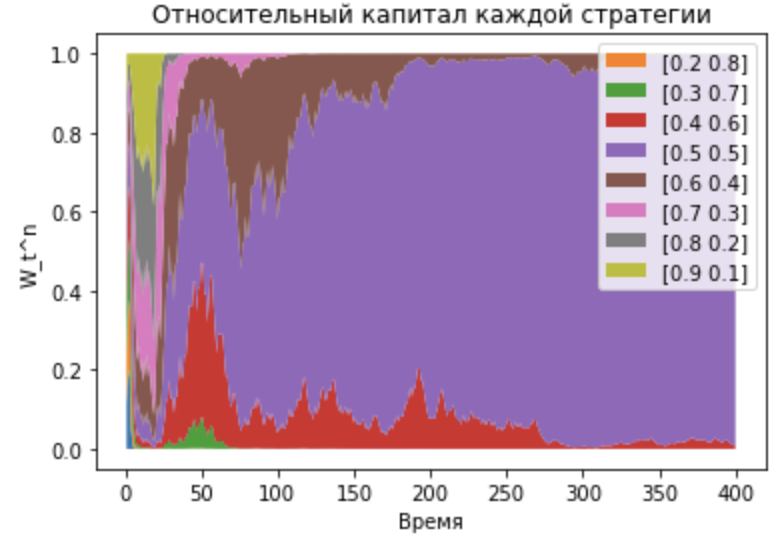
\includegraphics[height=4.25cm]{pictures/pic1-relative-wealth-all.png}\quad
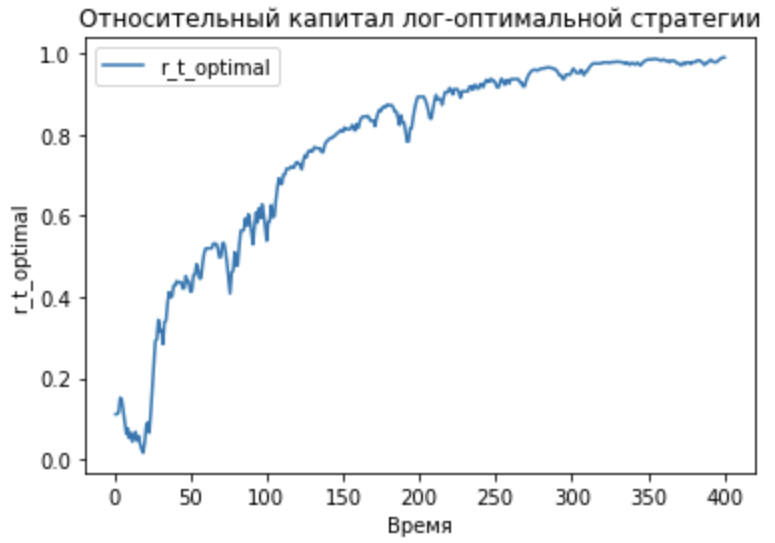
\includegraphics[height=4.25cm]{pictures/pic2-relative-wealth-optimal.png}\par
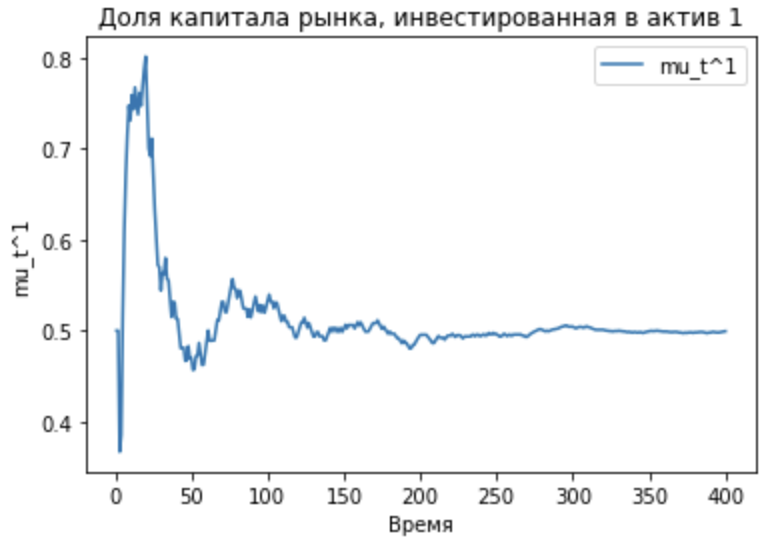
\includegraphics[height=4.25cm]{pictures/pic3-mut1-fraction.png}

\caption{\label{fig1} Эволюция капиталов агентов в одной симуляции рынка длиной в 400 шагов.
Слева сверху: относительные капиталы стратегий $\Lambda^n=(n/10, 1-n/10)$.
Справа сверху: относительный капитал оптимальной стратегии $\Lambda^*$.
Снизу: доля $\mu_{t}^1$ от капитала рынка, вложенная в первый актив.}
\end{figure}










%-------------------------------------------------------------------------------------------
\section{Связь с другими моделями}
\label{section5-relation-to-other-models}
Убедимся, что в рамках нашей модели можно получить известные для других, менее общих моделей, результаты про лог-оптимальные и выживающие стратегии.

В первой части этого раздела мы рассмотрим эволюционную финансовую модель с короткоживущими активами, предложенную в \cite{Amir2013}. В этой модели размеры дивидендов $A_t^k$ являются экзогенными, то есть зависят только от случайного фактора $s_t$, но не зависят от истории игоры (то есть от стратегий игроков $\bar\lambda_{t-1} =(\lambda_0, \dots, \lambda_{t-1})$).\\

Во второй части мы рассмотрим классическую модель рынка с экзогенными ценами активов, в которой действия агентов не влияют на цены активов и на капитал остальных агентов.


\subsection{ Модель с экзогенными размерами дивидендов.} 


Предположим, что в нашей молели $b_t^k=0$, и $a_t^k=a_t^k(\bar s_t)$ — зависит только от случайных состояний, но не зависит от стратегий агентов и начальных капиталов, то есть дивиденды $A_t^k=A_t^k(\bar s_t) = a_t^k(\bar s_t)$. Тогда уравнение динамики капитала \eqref{5-dynamics-of-W} превращается в 
\[
w_{t+1}^n = \sum_{k=1}^K 
\frac{\lambda_{t}^{n,k} W_t^n}{\sum_{n=1}^N \lambda_{t}^{n,k} W_t^n} a_{t+1}^k.
\]

Тогда, согласно нашим результатам, единственной стратегией, удовлетворяющей условиям \eqref{12-lambda-star-g}-\eqref{14-lambda-star-fixed-point} из Предложения~\ref{lemma2-lambda-star}, явлается \[
\Lambda_{t}^{*,k}(\bar s_t) 
= \E_t\left(\frac{a_{t+1}^k(\bar s_{t+1})}{\sum_{k=1}^K a_{t+1}^k(\bar s_{t+1})}\right),
\]
где $\Lambda^*_0$ — константный вектор. 
Эта стратегия распределяет капитал между активами пропорционально условным математическим ожиданиям их относительных дивидендов. Свойство выживаемости этой стратегии впервые было доказано в работе \cite{Amir2013}. Однако при дополнительных ограничениях на величины дивидендов $A_{t}^k$ оно было известно и ранее, см. \cite{BlumeEasley1992, AmirEvstigneev2005, Evstigneev2002}.


\subsection{Классическая модель с экзогенными ценами.}
Рассмотрим модель рынка с экзогенными ценами активов $S_{t}^k(\bar s_t)>0$, 
как в классической модели без коротких продаж  (см. \cite[Гл.~5]{FollmerSchied2011}). Мы покажем, что эта модель рынка является частным случаем нашей модели, а построенная в Теореме~\ref{theorem1-main} лог-оптимальная стратегия максимизирует ожидаемый логарифм капитала агента (или, что то же самое, логарифм доходности портфеля).

Как следствие, мы получаем новое свойство стратегии, максимизирующей ожидаемый логарифм капитала: она является неподвижной точкой отображения \eqref{14-lambda-star-fixed-point}.

Обозначим за  $X_{t+1}^k = S_{t+1}^k/S_{t}^k$ доходности активов.
Тогда эволюция капитала $W_t$ агента, использующего стратегию $\Lambda = \Lambda_t(\bar s_t)$ определяется соотношением
\[
W_{t+1} = W_t \langle \Lambda_t, X_{t+1}\rangle,
\]
где $\langle\,\cdot\,,\cdot\,\rangle$ обозначает скалярное произведение.
Эта модель получится как частный случай нашей модели, если в \eqref{6-A-t-k-affine} положить 
\begin{equation}
\label{17-beta-exogenous}
\alpha_{t+1}^k = 0, \qquad \beta_{t+1}^k = W_t X_{t+1}^k,
\end{equation}
где $W_t$ обозначает полный капитал рынка (Замечание~\ref{remark-abs-wealth} показывает, что  \eqref{17-beta-exogenous} можно записать в терминах $\mu_{t}^k$).

Напомним, что лог-оптимальная стратегия $\Lambda^*$ в классической теории роста капитала — это стратегия, максимизирующая ожидаемый логарифм доходности портфеля в каждый момент времени, то есть 
\begin{equation}
\label{18-log-max}
\Lambda_t^*(\bar s_t) 
\in \argmax_{\lambda\in \Delta^K} 
  \E_t \ln\langle \lambda, X_{t+1}(\bar s_{t+1})\rangle.
\end{equation}
Эта стратегия называется \emph{Kelly portfolio rule}.
Эта оптимизационная задача может не иметь решения, если лог-доходности не интегрируемы. Но если мы введем  \emph{относительные доходности}
\[
R_{t}^k = \frac{X_{t}^k}{\sum_{k=1}^K X_{t}^k}, \quad k=1,\dots,K,
\]
то, согласно классическому результату \cite{AlgoetCover1988}, лог-оптимальная стратегия будет являться решением задачи максимизации логарифмов относительных доходностей
\begin{equation}
\label{19-rel-log-max}
\Lambda^*_t(\bar s_t) 
\in \argmax_{\lambda\in \Delta^K} 
  \E_t \ln\langle \lambda, R_{t+1}(\bar s_{t+1})\rangle.
\end{equation}
В частности, задача \eqref{19-rel-log-max} всегда имеет решение при условии, что 
$\sum_{n=1}^N R_t^n > 0$ п.н. (однако решение может быть неединственно, если, например, $R_t^n$ линейно зависимы), и если задача  \eqref{18-log-max} имеет хотя бы одно регение, тогда множество решений задач \eqref{18-log-max} и \eqref{19-rel-log-max} совпадают. 

Исследуем связь между теми стратегиями, которые удовлетворяют условиям \eqref{12-lambda-star-g}--\eqref{14-lambda-star-fixed-point} в нашей модели, и классическими лог-оптимальными стратегиями\eqref{19-rel-log-max}. 
Отметим, что условие \eqref{12-lambda-star-g} выполняется для любой стратегии в этой модели, поскольку это условие эквивалентно условию
\[
\P_t(W_t \langle \Lambda_t^*, X_{t+1}\rangle = 0) = 0,
\]
которое, очевидно, выполнено, поскольку $X_{t+1}^k>0$. 
Условия \eqref{13-lambda-star-inequality} and \eqref{14-lambda-star-fixed-point} эквивалентны, соответственно, следующим условиям:
\begin{align}
\label{20-exogenous-conditions-1}
&\E_t\left(\frac{R_{t+1}^k}{\langle \Lambda_t^*, R_{t+1}\rangle}\right) \le 1, \\
\label{21-exogenous-conditions-2}
&\E_t\left(
  \frac{\Lambda_{t}^{*,k} R_{t+1}^k}{\langle \Lambda_t^*, R_{t+1}\rangle}
\right)
= \Lambda_{t}^{*,k}.
\end{align}
Легко видеть, что из \eqref{20-exogenous-conditions-1} следует \eqref{21-exogenous-conditions-2}.
Действительно, домножая обе части \eqref{exogenous-conditions-1} на $\Lambda_{t,k}^*$, мы получаем неравенство $\E_t\left(
  \frac{\Lambda_{t}^{*,k} R_{t+1}^k}{\langle \Lambda_t^*, R_{t+1}\rangle}
\right)
\le \Lambda_{t}^{*,k}$, в котором должно быть равенство с верояностью один, потому что иначе, суммируя обе части по $k=1,\dots,K$, мы получаем противоречие $1<1$ с положительной вероятностью.


Таким образом, в частном случае рассматриваемой модели, условия \eqref{12-lambda-star-g}--\eqref{14-lambda-star-fixed-point} эквивалентны условию \eqref{20-exogenous-conditions-1}.

\begin{proposition}
\label{prop3-maximaize-logreturns}
 Стратегия $\Lambda^* = \Lambda^*_t(\bar s_t)$  является $($ измеримым$)$ решением максимизационной задачи~\eqref{19-rel-log-max} тогда и только тогда, когда она удовлетворяет условиям \eqref{12-lambda-star-g}--\eqref{14-lambda-star-fixed-point} из Предложения~\ref{lemma-lambda-star} $($или, эквивалентно, условию \eqref{20-exogenous-conditions-1}$)$.
\end{proposition}

\begin{proof}
$ \Rightarrow$ Если стратегия  $\Lambda^*$ удовлетворяет условию \eqref{20-exogenous-conditions-1}, тогда для любой другой стратегии  $\Lambda = \Lambda_t(\bar s_t)$, пользуясь неравенством $\ln x \le x-1$, имеем:
\begin{multline*}
\E_t \ln\langle\Lambda_t,R_{t+1}\rangle 
  - \E_t \ln\langle\Lambda_t^*,R_{t+1}\rangle
= \E_t\ln\left( 
  \frac{\langle\Lambda_t,R_{t+1}\rangle}
       {\langle\Lambda_t^*,R_{t+1}\rangle}
\right) 
\le \E_t\left( 
  \frac{\langle\Lambda_t,R_{t+1}\rangle}
       {\langle\Lambda_t^*,R_{t+1}\rangle}
\right) - 1 =\\
= \left\langle \Lambda_t,
  \ \E_t\left(\frac{R_{t+1}}{\langle\Lambda_t^*,R_{t+1}\rangle}\right) 
\right\rangle - 1
=  \left\langle \Lambda_t,
  1 \right\rangle - 1=
\sum_{k=1}^K \Lambda_{t}^k - 1 = 0.
\end{multline*}

$ \Leftarrow$
Если стратегия $\Lambda_t^*$ является решением задачи \eqref{19-rel-log-max}, тогда известно (см. \cite[Т.~1]{AlgoetCover88}), что для любой стратегии $\Lambda$:
\[
\E_t \frac{\langle \Lambda_t, R_{t+1}\rangle}{\langle \Lambda_t^*, R_{t+1}\rangle} \le 1.
\]
Подставляя $\Lambda_t = (0,\dots,1,\dots,0)$ , получаем \eqref{20-exogenous-conditions-1}. 
\end{proof}





%----------------------------------------------------------------------------------------------
\section{Доказательства основных результатов}
\label{section6-proofs}
\subsection{Вспомогательные результаты}
Сначала докажем несколько вспомогательных лемм, которые потребуются для доказательства основных результатов.


\begin{lemma}
\label{lemma1-fixed-point}
Пусть $C\subset\R^K$ — компактное множество, а $(\Omega,\F)$ — измеримое пространство.
Пусть функция $L(x,\omega)\colon C\times\Omega\to C$ непрерывна по $x$ и измерима по $\omega$.

Тогда $L$ имеет измеримую неподвижную точку $\xi(\omega)$, то есть \ $L(\xi(\omega),\omega) = \xi(\omega)$ для всех $\omega\in\Omega$. 
\end{lemma}

\begin{proof}
Для каждого фиксированного $\omega\in\Omega$, неподвижная точка $\xi$ отображения $L(x,\omega)$ существует по теореме Брауэра.
Поэтому случайное множество $\Gamma(\omega) = \{x\in C : L(x,\omega)=x\}$ непусто для каждого $\omega$.

По теореме Куратовского-Рыля (см.\cite[ Т.~18.13]{Aliprantis2006}), это случайное множество является слабо измеримым \footnote{Мы называем случайное множесто $\Gamma\colon\Omega\to 2^{\R^K}$ \emph{слабо измеримым}, если  $\{\omega : \Gamma(\omega)\cap A \neq \emptyset\} \in \F$ для любого открытого $A\subset \R^K$.} и допускает измеримый селектор $\xi(\omega)\in \Gamma(\omega)$. Это и дает искомую измеримую неподвижную точку. 
\end{proof}


\begin{lemma}
\label{lemma2-convergent-subsequence}
Пусть $L^{n}(\omega)$, $n=1,2,\dots$ — последовательность измеримых функций на измеримом пространстве $(\Omega,\F)$ со значениями в компактном множестве $C\subset\R^K$.
Тогда существует измеримая функция $L^*(\omega)$ и строго возрастающая последовательность целочисленных измеримых функций $n_i(\omega)\ge 1$, $i=1,2,\dots$, таких что $\lim_{i\to\infty}L^{n_i(\omega)}(\omega) = L^*(\omega)$ для всех $\omega$. 
\end{lemma}

% \begin{proof}
% This result follows from Lemma~2 in \cite{KabanovStricker01}.
% \end{proof}

%% Alternative proof %%%
\begin{proof}
По теореме Кастена (см. Предложение 18.14 in \cite{Aliprantis2006}), непустое замкнутое случайное множество слабо измеримо тогда и только тогда, когда оно может быть представлено как замыкание счетного числа измеримых селекторов из этого отображения.
Следовательно, случайные множества $\Gamma^n = \mathrm{cl}\{L^k,\; k\ge n\}$, $n\ge1$ слабо измеримы.
Поскольку счетное пересечение компактных слабо измеримых случайных множеств слабо измеримо, то $\Gamma(\omega) = \bigcap_{n\ge 1}\Gamma^n(\omega)$ слабо измеримо.
Более того, $\Gamma(\omega)$ непусто, поскольку содержит предельную точку некоторой подпоследовательности $L^n(\omega)$.
Тогда по теореме Кастена существует измеримый селектор $L^*(\omega) \in \Gamma(\omega)$.

Тогда нужная последовательность $n_i$ может быть построена по индукции следующим образом.
Пусть $n_1=1$.
Если $n_i$ уже определено для некоторого $i\ge 1$, то рассмотрим случайное множество $\Psi_i(\omega) = \{k> n_i(\omega) : \|L^k(\omega) - L^*(\omega)\| \le i^{-1}\}$. Оно слабо измеримо, непусто и замкнуто.
Пучть $n_{i+1}$ — измеримый селектор из $\Psi_i$.
Тогда $\|L^{n_{i+1}} - L^*\| < \frac{1}{i}$, что дает искомую сходимость.
\end{proof}




\begin{lemma}
\label{lemma3-logsum}
Пусть $\alpha,\beta\in\R_+^N$ — два вектора, такие что
$\sum_n \alpha^n \le 1$, $\sum_n \beta^n \le 1$ и для всех $n=1,\ldots,N$ выполнено, что если $\beta^n=0$, то $\alpha^n=0$. Тогда верно следующее:
\begin{equation}
\sum_{n=1}^N\alpha^n \ln\frac{\alpha^n}{\beta^n} \ge
\frac{\|\alpha-\beta\|^2}{4} + \sum_{n=1}^N (\alpha^n-\beta^n),\label{logsum-1}
\end{equation}
где полагаем $\alpha^n \ln\frac{\alpha^n}{\beta^n} = 0$ если $\alpha^n=0$ или $\beta^n=0$.
\end{lemma}

\begin{proof}
Используя неравенство $-\ln x \ge 2(1-\sqrt x)$ для всех $x>0$, мы получем
\[
\begin{split}
\sum_{n=1}^N \alpha^n \ln\frac{\alpha^n}{\beta^n} &= -\sum_{n\,:\,\alpha^n\neq 0}\alpha^n\ln\frac{\beta^n}{\alpha^n} \ge
2\sum_{n=1}^N (\alpha^n-\sqrt{\alpha^n\beta^n}) \\&= \sum_{n=1}^N(\sqrt{\alpha^n} -
\sqrt{\beta^n})^2 + \sum_{n=1}^N (\alpha^n - \beta^n).
\end{split}
\]
Тогда мы можем использовать неравенство $(\sqrt x - \sqrt y)^2 \ge (x-y)^2/4$, которое верно для всех $x,y\in[0,1]$, и получить \eqref{logsum-1}. 
\end{proof}


Последняя лемма — это классический результат из теории мартингалов (чтоограниченный сверху обобщенный субмартингал 
\footnote{Напомним, что последовательность $S_t$ называется обобщенным субмартингалом, если $\E |S_0|<\infty$ и $\E(S_t\mid\F_{t-1})\ge S_{t-1}$ для всех $t\ge 1$ (но необязательно $\E|S_t|<\infty$). В Лемме~\eqref{lemma4-submart} доказывается, что если $S_t\le C$ для всех $t$, то $S_t$ интегрируемо и, следовательно, является настоящим субмартингалом.} является субмартингалом).


\begin{lemma}
\label{lemma4-submart}
Пусть $\zeta_t=\zeta_t(\bar s_t)$, $t=0,1,\dots$ ($\zeta_0$ константа)  — равномерно ограниченная сверху случайная последовательность (то есть\ $\zeta_t\le c$ п.н.\ для всех $t$ и некоторой константы $c$) и $\E_{t-1} \zeta_t\ge \zeta_{t-1}$ п.н.\ для всех $t\ge 1$.
Тогда $\E|\zeta_t| < \infty$, то есть $\zeta_t$ — настоящий субмартингал.
\end{lemma}
\begin{proof}
Последовательность $M_t$ с $M_0=0$ и
\[
M_t = \zeta_t - \sum_{s=1}^t (\E_{t-1} \zeta_t - \zeta_{t-1}),\quad
t \ge 1,
\]
является локальным мартингалом, поскольку $\E_{t-1} M_t = M_{t-1}$ \cite[Гл.~7.1, Т.~1]{Shiryaev2019}.
Поскольку она ограничена сверху, эта последовательность является настоящим мартингалом  \cite[Гл.~7.1, Т.~3]{Shiryaev2019}, поэтому $\E |M_t| < \infty$.
Используя тот факт, что $M_t \le \zeta_t \le c$, получаем $\E|\zeta_t| < \infty$. 
\end{proof}

\begin{lemma}
\label{lemma5-compensator}
Пусть $X_t$, $t=0,1,\dots$ — процесс в дискретном времени. Тогда его компенсатор имеет вид
\[
A_t := \sum_{i=0}^{t-1} (\E_{i} X_{i+1} - X_i)
\]
\end{lemma}

\begin{proof}
Пусть $A_{t}$ — компенсатор для $X_t$, то есть $A_t$ — предсказуемая последовательность, и $X_{t+1} - A_{t+1}$ — мартингал.
Тогда 
\[
\E_{t} \left(  X_{t+1} - A_{t+1} \right) = X_t - A_t
\]
Следовательно, 
\[
E_{t} X_{t+1}  -X_t = A_{t+1} - A_t
\]
Отсюда получаем формулу для $A_t$:
\[
A_t := \sum_{i=0}^{t-1} (\E_{i} X_{i+1} - X_i)
\]


\end{proof}

\subsection{Доказательство Предложения~\ref{lemma2-lambda-star} о неподвижной точке}
\begin{proof}
Зафиксируем $t\ge 0$.
Введем $\Delta^K$-значные функции $g_{t,n}(\lambda^*, \bar s_t, \bar\chi_{t-1})$ и $L_{t,n}(\lambda^*, \bar s_t, \bar\chi_{t})$, $n=1,2,\dots$, следующим образом:
\begin{gather*}
g_{t,n}^k = g_{t}^k + \frac 1 n,\\
L_{t,n}^k(\lambda^*, \bar s_t,\bar\chi_t) = \E_t\left(
  \frac{g_{t+1,n}^k(\lambda^*,\bar s_{t+1}, \bar\chi_t)}
       {\sum_{k=1}^K g_{t+1,n}^k(\lambda^*, \bar s_{t+1}, \bar\chi_t)} 
  \right).
\end{gather*}
Напомним, что $\E_t(\cdot)$ обозначает условное ожидание относительно зафиксированного варианта регулярного условного распределения $\bar s_{t+1}$. Функции $L^n_t$ непрерывны по $\lambda^*\in \Delta^K$ и измеримы по $(\bar s_t, \bar\chi_{t})$.
Тогда по Лемме~\ref{lemma1-fixed-point} у них есть измеримые неподвижные точки $\Lambda_{t,n} = \Lambda_{t,n}(\bar s_t, \bar\chi_t)$, то есть для любых $(\bar s_t,\bar \chi_t)$ выполнено
\begin{equation}
\label{23-Ln-fp}
L_t^n(\Lambda_t^n(s^t,\chi^t), s^t, \chi^t)
= \Lambda_t^n(s^t,\chi^t).
\end{equation}
Пусть
\[
\delta_{t,n}^k(\bar s_t,\bar\chi_t) 
= \E_t \left(
  \frac{b_{t+1}^k( \bar s_{t+1}, \bar\chi_t)}
       {\sum_{k=1}^K 
         g_{t+1,n}^k(\Lambda_{t,n}(\bar s_t, \bar\chi_t), \bar s_{t+1}, \bar\chi_t)}
  \right).
\]
Заметим, что 
\begin{equation}
\label{24-delta-1}
\delta_{t,n}^k \le 1, \quad k=1,\dots,K,
\end{equation}
поскольку
\[
(1-\delta_{t,n}^k)\Lambda_{t,n}^k 
= \E_t\left( 
  \frac{a_{t+1}^k + 1/n}
       {\sum_{k=1}^K g_{t+1,n}^k(\Lambda_{t,n})}
  \right) > 0.
\]
По лемме~\ref{lemma2-convergent-subsequence}, можно найти возрастающую последовательность $n_i = n_i(\bar s_t, \bar\chi_t)$, $i=1,2,\dots$ такую, что существует предел
\[
\Lambda^*_{t} = \lim_{i\to\infty} \Lambda_{t,n_i}
\]
Теперь, для фиксированного $\bar \chi_t$, переходя к пределу$i\to\infty$ и $n_i\to\infty$ в \eqref{24-delta-1} (используя лемму Фату и предположение \eqref{9-a-b-assumption}), получаем, что \eqref{12-lambda-star-g} выполнено.
Далее, по теореме Лебега о мажорируемой сходимости получаем \eqref{13-lambda-star-inequality} из \eqref{24-delta-1} и \eqref{14-lambda-star-fixed-point} из \eqref{23-Ln-fp}.

\end{proof}




\subsection{Доказательство Теоремы~\ref{theorem1-main}}

\begin{proof}
Зафиксируем вектор начальных капиталов и профиль стратегий, в котором один агент использует старетегию $\Lambda^*$.
Без потери общности, предположим, что стратегию $\Lambda^*$ использует агент 1. 

Введем обозначение (опуская зависимость от $\bar s_t$ для краткости) 
\[
\theta_{t}^k = \frac{\lambda_{t}^{1,k}}{\mu_{t}^k}.
\]

Напомним, что 
\[
W_t = \sum_{n=1}^N W_t^n, \qquad
\mu_{t}^k = \frac{1}{W_t}\sum_{n=1}^{N}\lambda_{t}^{n,k} W_t^n.
\]

Тогда уравнение динамики капитала \eqref{5-dynamics-of-W} переписывается в виде
\[
W_{t+1}^1 = 
\sum_{k=1}^K \frac{\lambda_{t}^{n,k} W_t^n}{\sum_{n=1}^N \lambda_{t}^{n,k} W_t^n} A_{t+1}^k
=r_t^1 \sum_{k=1}^K \theta_{t}^k A_{t+1}^k 
= r_t^1\sum_{k=1}^K (\theta_{t}^k \alpha_{t+1}^k + \lambda_{t}^{1,k}\beta_{t+1}^k), 
\]
а полный капитал рынка удовлетворяет уравнению 
\[
W_{t+1} = \sum_{k=1}^K A_{t+1}^k 
= \sum_{k=1}^K (\alpha_{t+1}^k + \mu_{t}^k \beta_{t+1}^k).
\]

Поэтому 
\[
r_{t+1}^1 = \frac {W_{t+1}^1}{W_t}= \frac{r_t^1\sum_{k=1}^K (\theta_{t}^k \alpha_{t+1}^k + \lambda_{t}^{1,k}\beta_{t+1}^k)}{\sum_{k=1}^K (\alpha_{t+1}^k + \mu_{t}^k \beta_{t+1}^k)}
\]
Из последнего равенства получаем 
\begin{equation}
\label{25-log-r}
\ln r_{t+1}^1 - \ln r_t^1 
= \ln\Biggl(
  \frac{\sum_{k=1}^K (\theta_{t}^k \alpha_{t+1}^k + \lambda_{t}^{1,k}\beta_{t+1}^k)}
       {\sum_{k=1}^K (\alpha_{t+1}^k + \mu_{t}^k \beta_{t+1}^k)}
  \Biggr).
\end{equation}

Consequently, we can represent
\[
\E_t \ln r_{r+1}^1 - \ln r_t^1 = \E_t(F_{t+1} + G_{t+1}), 
\]
where
\begin{align}
\label{26-F}
&F_{t+1} = \ln \biggl(
  \frac{\sum_{k=1}^K (\theta_{t}^k\alpha_{t+1}^k + \lambda_{t}^{1,k}\beta_{t+1}^k)}
       {\sum_{k=1}^K (\alpha_{t+1}^k + \lambda_{t}^{1,k}\beta_{t+1}^k)}
  \biggr),\\
\label{27-G}
&G_{t+1} = \ln\biggl(
  \frac{\sum_{k=1}^K (\alpha_{t+1}^k + \lambda_{t}^{1,k} \beta_{t+1}^k)}
       {\sum_{k=1}^K (\alpha_{t+1}^k + \mu_{t}^k \beta_{t+1}^k)}
  \biggr).
\end{align}

Покажем, что $\E_{t}(F_{t+1} + G_{t+1}) \ge 0$.
Рассмотрим аргумент логарифма в \eqref{26-F} как выпуклую комбинацию чисел
\[
\theta_{t}^k,\ \ldots ,\ \theta_{t}^K, 1
\]
с коеффициентами
\[
\frac{\alpha_{t+1}^k}
     {\sum_{k=1}^K(\alpha_{t+1}^k + \lambda_{t}^{1,k}\beta_{t+1}^k)},
       \ k=1,\dots,K, \qquad
\frac{\sum_{k=1}^K \lambda_{t}^{1,k}\beta_{t+1}^k}
     {\sum_{k=1}^K(\alpha_{t+1}^k + \lambda_{t}^{1,k}\beta_{t+1}^k)}.
\]
Из-за выпусклости вверх логарифма получаем:
\begin{equation}
\label{28-F-bound}
F_{t+1} 
\ge \sum_{k=1}^K
  \frac{\alpha_{t+1,k}}
       {\sum_{k=1}^K (\alpha_{t+1}^k + \lambda_{t}^{1,k} \beta_{t+1}^k)}
  \ln \theta_{t}^k.
\end{equation}

Обозначим за 
\begin{equation}
\label{29-gamma-t-k}
\gamma_{t}^k 
= 1 
  - \E_t \left( 
    \frac{\beta_{t+1}^k}
         {\sum_{k=1}^K (\alpha_{t+1}^k + \lambda_{t}^{1,k} \beta_{t+1}^k)}
  \right),
  \qquad k=1,\dots,K.

\end{equation}

Из \eqref{13-lambda-star-inequality}, мы имеем $\gamma_{t}^k\in [0,1]$, а из \eqref{14-lambda-star-fixed-point} следует, что 
\begin{equation}
\label{gt-lambda}
\gamma_{t}^k \lambda_{t}^{1,k} 
= \E_t \left(
  \frac{\alpha_{t+1}^k}
       {\sum_{k=1}^K(\alpha_{t+1}^k + \lambda_{t}^{1,k} \beta_{t+1}^k)}
  \right).
\end{equation}

Беря ожидание в \eqref{28-F-bound}, получаем
\begin{multline}
\label{31-EF-bound}
\E_t F_{t+1} 
\ge \sum_{k=1}^K \gamma_{t}^k \lambda_{t}^{1,k} \ln \theta_{t}^k 
= \sum_{k=1}^K \gamma_{t}^k \lambda_{t}^{1,k} 
  \ln\frac{\gamma_{t}^k\lambda_{t}^{1,k}}{\gamma_{t}^k\mu_{t}^k} \\
\ge \frac 14\sum_{k=1}^K (\gamma_{t}^k(\lambda_{t}^{1,k} - \mu_{t}^k))^2 
  + \sum_{k=1}^K \gamma_{t}^k(\lambda_{t}^{1,k} - \mu_{t}^k),
\end{multline}
где во втором неравенстве мы применили Лемму~\ref{lemma3-logsum} к векторам $\alpha,\beta$ с координатами
\[
\alpha_k = \gamma_{t}^k\lambda_{t}^{1,k}, \qquad \beta_k = \gamma_{t}^k\mu_{t}^k.
\]
Отметим, что условия $\sum_{k=1}^K \alpha_k \le 1$, $\sum_{k=1}^K \beta_k \le 1$ из леммы выполнены, так как векторы $\lambda_t^1$ and $\mu_t$ сами удовлетворяют этому свойству, а $\gamma_{t}^k \in [0,1]$.

Для оценки снизу $\E_t G_{t+1}$, мы используем неравенство $\ln a \ge 1 - a^{-1}$ и получаем
\begin{multline}
\label{32-EG-bound}
\E_t G_{t+1} 
\ge \E_t \left( 
  \frac{\sum_{k=1}^K (\lambda_{t}^{1,k} - \mu_{t}^k) \beta_{t+1}^k}
       {\sum_{k=1}^K (\alpha_{t+1}^k + \lambda_{t}^{1,k} \beta_{t+1}^k)}
  \right) \\
= \sum_{k=1}^K (1-\gamma_{t}^k) (\lambda_{t}^{1,k} - \mu_{t}^k) 
= \sum_{k=1}^K \gamma_{t}^k (\mu_{t}^k - \lambda_{t}^{1,k}),
\end{multline}
где последнее равенство получается из-за того, что $\sum_{k=1}^K \lambda_{t,k}^1 = \sum_{k=1}^K \mu_{t,k} = 1$. 

Из оценок \eqref{31-EF-bound} и \eqref{32-EG-bound} получаем:
\begin{equation}
\label{33-compensator-bound}
\E_t(F_{t+1}+G_{t+1}) 
\ge \frac14 \sum_{k=1}^K (\gamma_{t}^k(\lambda_{t}^{1,k} - \mu_{t}^k))^2,
\end{equation}
so $\E_t (F_{t+1}+G_{t+1})\ge 0$.
По Лемме ~\ref{lemma4-submart}, оценивая $\ln r_t^1$ сверху нулем, получаем, что $\ln r_t^1$ субмартингал. 

\end{proof}

\subsection{Доказательство Теоремы~\ref{theorem2-convergence}}
Предположим, что стратегию $\Lambda^*$ использует агент 1.
В ходе доказательства Теоремы~\ref{theorem1-main}, мы показали, что $\zeta_t:=\ln r_t^1$ является субмартингалом,так как $\E_{t}\ln r_{t+1}^1 - \ln r_{t}^1=F_t + G_t \geq 0$ . 

Применяя разложение Дуба, получаем $\zeta_t = \zeta_0 + M_t + A_t$, где $M_t$ — мартингал, $A_t$ — предсказуемая неубывающая последовательность (\emph{компенсатор} $\zeta_t$), и $M_0=A_0=0$.

При этом $r_t^1 \leq 1$, а значит, $\ln r_t^1 \leq 0$, то есть $\ln r_t^1$ является ограниченным субмартингалом. По следствию из теоремы Дуба о сходимости, этот субмартингал сходится.

Но поскольку ограниченный субмартингал $\zeta_t$ сходится к конечному пределу при $t\to\infty$, то и его компенсатор имеет конечный предел, другими словами, \ $\lim_{t\to\infty} A_t < \infty$ п.н.

Из формулы для компенсатора из Леммы~\ref{lemma5-compensator} и оценки \eqref{33-compensator-bound} получаем
\[
A_t := \sum_{u=0}^{t-1} (\E_u\zeta_{u+1} - \zeta_u) 
\ge \frac14 \sum_{u=0}^{t-1} 
  \sum_{k=1}^K (\gamma_{u}^k(\lambda_{u}^{1,k} - \mu_{u}^k))^2.
\]
Тогда из условия \eqref{15-lambda-star-inequality-strong} Теоремы~\ref{theorem2-convergence} и соотношения \eqref{29-gamma-t-k}, получаем, что $\gamma_{t}^k\ge \epsilon>0$.
Теперь утверждение теоремы следует из сходимости $A_t$.





\subsection{Доказательство Теоремы~\ref{theorem3-iid}}
(a) Существование константной стратегии, удовлетворяющей условиям \eqref{12-lambda-star-g}--\eqref{14-lambda-star-fixed-point}, (а следовательно, являющейся лог-оптимальной), следует из доказательства Утверждения~\ref{lemma2-lambda-star}.

(b) Пусть предположение \eqref{16-iid-a-positive} выполнено.
Пусть
\begin{equation}
\label{gt-iid}
\gamma^k 
= 1 - \E\left( \frac{b^k(s_t)}{\sum_{k=1}^K (a^k(s_t) + \Lambda^{*,k} b^k(s_t))}\right),
  \qquad k=1,\dots,K.
\end{equation}
Тогда из \eqref{14-lambda-star-fixed-point} получаем
\begin{equation}
\label{gt-lambda-iid}
\gamma_k \Lambda^{*,k} 
= \E \left(
  \frac{a^k(s_t)}
       {\sum_{k=1}^K(a^k(s_t) + \Lambda^{*,k} b^k(s_t))}
  \right),
\end{equation}
поэтому $\gamma_k\Lambda^{*,k}>0$, а значит, $\gamma^k>0$, то есть условие \eqref{15-lambda-star-inequality-strong} выполнено.
Из Теоремы~\ref{theorem2-convergence}, мы получаем сходимость $\mu_t\to\Lambda^*$.

Если $\tilde\Lambda\in \Delta^K$ — другая выживающая стратегия, то она обязана выживать в профиле стратегий $(\tilde\Lambda, \Lambda^*,\dots,\Lambda^*)$.

Это значит, что $\inf_{t\ge 0} r_t^1 > 0$ п.н.

Но тогда сходимость $\mu_t = r_t^1\tilde\Lambda + (1-r_t^1)\Lambda^* \to \Lambda^*$ имеет место только при $\tilde\Lambda = \Lambda^*$.
Следовательно, $\Lambda^*$ — единственная выживающая стратегия.

(c) Рассмотрим профиль стратегий, в котором агент 1 использует стратегию $\Lambda^*$.
Пусть агент $i$ использует константную стратегию $\Lambda^i\neq\Lambda^*$.
Для доказательства теоремы, мы должны показать, что $r_t^1/r_t^i \to \infty$ с вероятностью единица при $t\to\infty$.

Для этого мы покажем, что 
\begin{equation}
\label{36-liminf}
\liminf_{t\to\infty} t^{-1} \ln \frac{r_t^1}{r_t^i} > 0.
\end{equation}

Из равенства \eqref{25-log-r} в доказательстве Теоремы~\ref{theorem1-main}, после сокращения знаменателей в вычитаемых дробых получаем
\[
D_{t+1} := \ln\frac{r_{t+1}^1}{r_{t+1}^i} - \ln\frac{r_t^1}{r_t^i}= 
\ln\frac{r_{t+1}^1}{r_{t}^1} - \ln\frac{r_{t+1}^i}{r_t^i}
= \ln\Biggl(
  \frac{\sum_{k=1}^K(\theta^1_{t,k} \alpha_{t+1,k} + \Lambda^*_k\beta_{t+1,k})}
       {\sum_{k=1}^K(\theta^i_{t,k} \alpha_{t+1,k} + \Lambda^i_k\beta_{t+1,k})}
  \Biggr),
\]
где $\alpha_{t}^k = a^k(s_t)$, $\beta_{t}^k = b^k(s_t)$, и $\theta_{t}^{1,k} = \Lambda^{*,k}/\mu_{t}^k$, $\theta_{t}^{i,k} = \Lambda^{i,k}/\mu_{t}^k$. 

Тогда получаем
\[
t^{-1} \ln \frac{r_t^1}{r_t^i} 
= t^{-1}\ln\frac{r_0^1}{r_0^i} + t^{-1}\sum_{u=0}^{t-1} \E_u D_{u+1} 
  + t^{-1}\sum_{u=0}^{t-1} (D_{u+1} - \E_u D_{u+1}).
\]
Заметим, что последовательность $D_t$ равномерно ограничена:
\[
\frac{1}{c} \le D_t < c,
\]
где $c=\max_{i,k} \Lambda^{i,k}/ \min_{i,k} \Lambda^{i,k}$.

Из усиленного закона больших чисел для мартингалов, получаем п.н. сходимость
$$\xi_t := t^{-1} \sum_{u=0}^{t-1} (D_{u+1} - \E_u D_{u+1}) \to 0 $$

Значит, для того, чтобы получить \eqref{36-liminf}, достаточно показать, что существует  $\epsilon>0$ и случайный момент времени $\tau$ такой, что для $t\ge \tau$ выполнено
\begin{equation}
\label{37-Dlim}
\E_t D_{t+1} \ge \epsilon.
\end{equation}

Согласно Теореме~\ref{theorem1-main}, мы имеем $\mu_{t,k} \to \Lambda^{*,k}$, поэтому $\theta_{t}^{1,k} \to 1$ и $\theta_{t}^{i,k} \to \Lambda^{i,k}/\Lambda^{*,k}$.
Поэтому, с вероятностью единица, имеем
\[
\lim_{t\to\infty} \E_t D_{t+1} = \E \ln\Biggl(
  \frac{\sum_{k=1}^K (\alpha_k + \Lambda^{*,k}\beta^k)}
       {\sum_{k=1}^K (\Lambda^{i,k} \alpha_k/\Lambda^{*,k} + \Lambda^{i,k}\beta_k)}
  \Biggr) =: \E \ln \zeta,
\]
где $(\alpha,\beta)$ — пара векторов из $\R^K$ с таким же распределением, как и у  $(a(s_t), b(s_t))$.

Поэтому, чтобы получить \eqref{Dlim}, нам нужно показать $\E \ln \zeta >0$, или, что эквивалентно, $\E \ln \zeta^{-1} < 0$.
Используя строгую выпуклость вверх логарифма и неравенство Йенсена, достаточно показать, что $\E \zeta^{-1} = 1$ и $\zeta$ не константа п.н. \textcolor{red} { А почему важно, что не константа?} 

Для доказательства последнего утверждения, используем \eqref{gt-iid} и \eqref{gt-lambda-iid}, откуда получаем
\[
\E \zeta^{-1} = \E \Biggl(
  \frac{\sum_{k=1}^K (\Lambda^{i,k} \alpha_k/\Lambda^{*,k}+ \Lambda^{i,k}\beta^k)}
       {\sum_{k=1}^K (\alpha^k + \Lambda^{*,k}\beta^k)}       
  \Biggr) = \sum_{k=1}^K (\gamma_k\Lambda^{i,k} + (1-\gamma_k)\Lambda^{i,k}) = 1.
\]
Тот факт, что $\zeta$ не константа, следует из того, что  случайные величины $a_{t}^k/\Lambda^{*,k} + b_{t}^k$ линейно независимы. В самом деле, если $\zeta=c$, тогда 
\[
\sum_{k=1}^K (c\Lambda^{*,k} - \Lambda^{i,k}) \left( \frac{\alpha_k}{\Lambda^{*,k}} + \beta^k\right) = 0 ,
\]
откуда $c\Lambda^{*,k} = \Lambda^{i,k}$ для всех $k$, откуда $\Lambda^i=\Lambda^*$, что противоречит нашему предположению. 



%---------------------------------------------------------------------------------------------
\section{Заключение}
\label{section7-conclusion}

В работе сформулирована  и изучена модель рынка с дискретным временем, короткоживущими активами и эндогенными аффинными выплатами этих активов. Предложено определение выживающих стратегий, которые позволяют использующему их инвестору не быть вытесненным с рынка на бесконечном горизонте времени. 
В предложенной  модели, во-первых, найдено описание лог-оптимальной (а значит, выживающей) стратегии как неподвижной точки специального отображения (см. Теорему~\ref{theorem1-main}). 

Во-вторых, доказано, что лог-оптимальная стратегия определяет агрегированное поведение рынка на бесконечном горизонте времени в том смысле, что если в профиле стратегий какой-то агент использует лог-оптимальную стратегию, то (при немного более сильных требованиях к дивидендам) взвешенная на капиталы стратегия всех остальных агентов в этом профиле стратегий стремится в лог-оптимальной стратегии (см. Теорему~\ref{theorem2-convergence}).

 В третьих, доказано, что в случае независимых одинаково распределенных коеффициентах из афиинных функций, определяющих дивиденды, лог-оптимальная стратегия оказывается единственной выживающей стратегией в классе константных стратегий (см. Теорему~\ref{theorem3-iid}).

 Наконец, проведено сведение предложенной аффинной модели к классической модели с экзогенными выплатами и получена новая характеризация уже давно известной оптимальной стратегии в этой модели как неподвижной точки специоального отображения. Также проведено сведение предложенной аффинной модели к классической модели с экзогенными ценами активов и приведенотальтернативное доказательство того, что что лог-оптимальная стратегия макисимизирует логарифмы доходностей (см. Утвержднение~\ref{prop3-maximaize-logreturns}).

 Также написана программа на языке Python, позволяющая провести симуляции и наглядно увидеть на примере рынка с двумя активами, что оптимальная стратегия действительно завоевывает весь рынок на бесконечном горизонте времени.

 






%-------------------------------------------------------------------------------------------
\begin{thebibliography}{}
%\addcontentsline{toc}{section}{6 \; Список литературы}

\bibitem{AlgoetCover1988} Algoet, P. H. and Cover, T. M. (1988). 
\newblock Asymptotic optimality and asymptotic equipartition properties of log-optimum investment. 
\newblock {\em The Annals of Probability}, 16(2):876–898.


\bibitem{Aliprantis2006} Aliprantis C. D., and Border K. C. (2006).
\newblock Infinite Dimensional Analysis: A Hitchhiker’s Guide.
\newblock {\em Springer}, 3rd edition, 591–600.


\bibitem{Amir2013} Amir R., Evstigneev I. V., and Schenk-Hoppé, K. R. (2013).
\newblock Asset market games of survival: a synthesis of evolutionary and dynamic games.
\newblock {\em Annals of Finance}, 9(2):121–144.

\bibitem{AmirEvstigneev2005} Amir R., Evstigneev I. V., and Schenk-Hoppé, K. R. (2005).
\newblock Market selection and survival of investment strategies.
\newblock {\em Journal of Mathematical Economics}, 41(1-2):105-122.

\bibitem{BlumeEasley1992} Blume L. and Easley D. (1992).
\newblock Evolution and market behaviour.
\newblock {\em Journal of Economic Theory}, 58(1):9–40.


\bibitem{Breiman1961} Breiman, L. (1961). 
\newblock Optimal gambling systems for favorable games.
\newblock {\em Proceedings of the 4th Berkeley Symposium on Mathematical Statistics and Probability}, 1:63–68.


\bibitem{Bharucha-reid1976} Bharucha-Reid, A. T. (1976).
\newblock Fixed point theorems in probabilistic analysis. \newblock {\em Bulletin of the American Mathematical Society}, 82(5):641–657.


\bibitem{Drokin-Zhitlukhin2020} Drokin, Y. and Zhitlukhin, M. (2020).
\newblock Relative growth optimal strategies in an asset market game.
\newblock {\em Annals of Finance}, 16:529–546.


\bibitem{EvstigneevEvolFinance2016} Evstigneev, I., Hens, T., and Schenk-Hoppé, K. R. (2016).
\newblock Evolutionary behaviorial finance. In Haven, E. et al., editors, 
\newblock {\em The handbook of Post Crisis Financial Modelling}, 214-234. Palgrave Macmillan UK.

\bibitem{Evstigneev2002} Evstigneev, I., Hens, T., and Schenk-Hoppé, K. R. (2016).
\newblock Market selection of financial trading strategies: Global stability. 
\newblock {\em Mathematical Finance}, 12(4):329-339.

\bibitem{FollmerSchied2011} Föllmer, H. and Schied, A. (2011). 
\newblock {\em Stochastic Finance: an Introduction in Discrete Time}. Walter de Gruyter, Berlin/New York, 3rd edition.


\bibitem{Holfort2019} Holtfort, T. (2019). 
\newblock From standard to evolutionary finance: a literature survey. 
\newblock {\em Management Review Quarterly}, 69(2):207–232.


\bibitem{KaratzasKardaras2007} Karatzas, I. and Kardaras, C. (2007). 
\newblock The numeraire portfolio in semimartingale financial models. 
\newblock {\em Finance and Stochastics}, 11(4):447–493.


\bibitem{Kelly1956} Kelly, Jr, J. L. (1956). 
\newblock A new interpretation of information rate. 
\newblock {\em Bell System Technical Journal}, 35(4):917–926.

\bibitem{Shapley-Shubik1977} Shapley, L. and Shubik, M. (1977). 
\newblock Trade using one commodity as a means of payment.
\newblock {\em Journal of political economy}, 
    85(5):937-968.

\bibitem{Shiryaev2019} Shiryaev, A.N. (2019). 
\newblock Probability-2.
\newblock {\em Springer}, 
    3rd edition.
  
\end{thebibliography}

\end{document}



